\subsection{真实 Megakernel 的实验基础}

本课题以 Hazy Megakernels 作为可复现研究载体，版本和固定提交见公开仓库\cite{hazyMegakernels2025}。目标代码采用 Hopper 低时延 Llama 路径，实验复用上游 Attention、MatVec 与通用 VM task code。模型权重采用公开、同形的 Llama checkpoint，其版本由公开实现固定\cite{inferenceOptimization2025llama05b}。连续自然文本 token 序列由冻结的输入生成脚本产生。主实验中的一个 grid 包含 132 CTAs，每个 CTA 640 threads；worker 在运行时读取 SMID 并选择对应 instruction queue。

中心 A/B 将 \texttt{PartialAttention}\allowbreak{} $\rightarrow$ \allowbreak{}\texttt{O\_ProjResidual} 实现为一次或两次 \texttt{mk\_llama} launch。inside instruction tensor 等于 prefix 与 suffix tensor 在 slot 维的逐字节拼接；两种方案均包含 136 个真实 tasks、128 个 noops 和相同的 33,792 instruction bytes。attention output、hidden output 和 barrier 逐位一致，并通过独立 PyTorch reference。该控制使性能处理变量对应相同 isolated task stream 中间是否放置物理 grid boundary。

表~\ref{tab:preliminary-evidence} 汇总先导实验的控制条件与可识别结论。131K context 下，原始 Hazy binary 的三个独立进程均得到 $45.42$--$46.64\microsecond$ 的成对净节省；32K、65K、98K、120K 和 131K 扫描显示绝对差值随长 attention producer 从约 $7$--$8\microsecond$ 增长到约 $45$--$47\microsecond$。同一图的三条相邻边呈相反方向，构成边界选择的正负样本。

\begin{table}[htbp]
  \centering
  \small
  \caption{H800 先导实验的控制条件与直接结论}
  \label{tab:preliminary-evidence}
  \begin{tabularx}{\textwidth}{p{0.22\textwidth}p{0.39\textwidth}X}
    \toprule
    实验资产 & 已实施控制 & 可识别结论 \\
    \midrule
    Slot-exact 中心边
      & 固定 task code、queue 映射、输入输出、task/noop 位置和 33,792 instruction bytes
      & 原始 single-grid 与 serial split 的净差值来自物理映射变化 \\
    数值与同步正确性
      & Attention、hidden、barrier 逐位比较；独立 PyTorch reference；随机交错复用
      & A/B 保持算子数值语义与跨阶段依赖语义 \\
    独立重复
      & 131K 三个独立进程各 100 对；32K 中心边在第二张 H800 上复验；计时与 profiler 分离
      & 正边方向跨进程、跨卡保持；进程内噪声由 A/A 量化 \\
    动态 task 顺序
      & 124 个早到候选 queues 的 $372/372$ 次观测均在 full-ready 前进入依赖等待
      & 全量 readiness 与 SM-local 提前推进在真实执行中同时发生 \\
    first-TMA $\times$ backoff
      & 两张 H800、三个独立进程、四个 cells，共 12 个 paired medians
      & ready 前 weight TMA 与 polling load 数量均非维持 $44.832$--$47.776\microsecond$ 差距的单一主因 \\
    同边 Split+PDL
      & 一张物理 H800；修改后的匹配 binary；serial/PDL 仅改变 programmatic launch 路径
      & PDL 在该边进一步节省 $2.4$--$3.8\microsecond$，并形成真实 grid overlap \\
    \bottomrule
  \end{tabularx}
\end{table}

图~\ref{fig:context-split-gain}(a) 给出冻结 task stream 下长 context 的绝对收益范围。context 从 65K 增至 131K 时，物理分区节省从约 $20\microsecond$ 增至约 $46\microsecond$；120K Nsys 中可见 grid gap 为 $1.056\microsecond$。图~\ref{fig:context-split-gain}(b) 将同一 Hazy 计算图的四条相邻边统一到 32K workload：中心边的三个独立进程均支持物理分区，其余三条边均支持 single-grid 执行。绝对收益随 producer window 增长，而边界方向随依赖结构变化；两项观察共同确定后续 single-grid admission 与跨阶段交接实验的量级和对照组。

\begin{figure}[htbp]
  \centering
  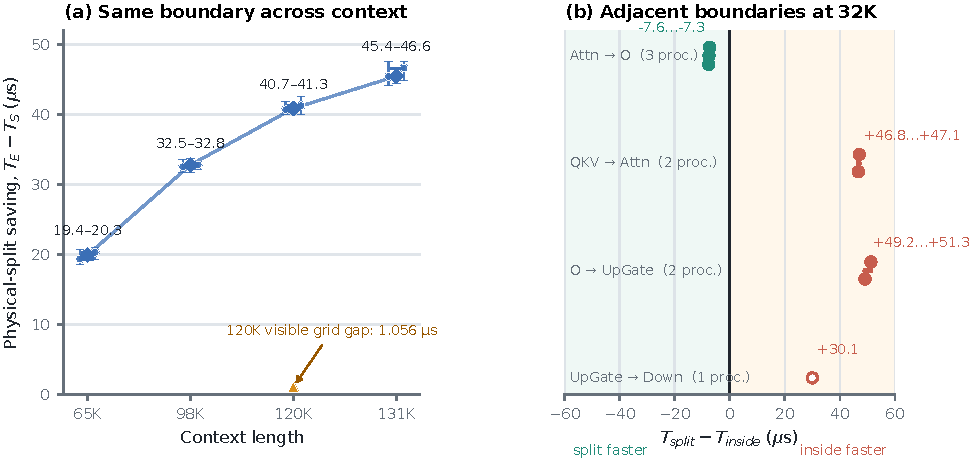
\includegraphics[width=0.98\textwidth]{Img/paper_figures/fig_h800_boundary_results.pdf}
  \caption{H800 上的物理边界实测结果。(a) 蓝色小点与细误差线表示各独立进程的 paired median 和进程内 paired-bootstrap 95\% 区间，菱形与粗短线表示进程间中位数和 min--max 范围；正值表示 Serial-Split 更快。橙色三角为 120K Nsight Systems 单独测得的可见 inter-grid gap。(b) 同一 32K workload 上四条相邻边的进程级 paired median；绿色区域对应 split 更快，红色区域对应 inside 更快，空心点表示该边当前包含一个独立进程。}
  \label{fig:context-split-gain}
\end{figure}

\subsection{SM、SASS 与关键路径分析基础}

源码审计已经确定中心边的依赖结构：8 个 PartialAttention tasks 产生 32 个 query heads，128 个 O-projection tasks 各自读取完整的 \texttt{attn\_out[2048]}。SASS 中已经定位 global ready counter 的 system-scope load、compare、nanosleep 回环、CTA barrier、weight TMA 和首次 activation load。逐 SM 时间戳进一步确认 queues 8--131 的实际提前进入与 first-TMA 顺序。

Nsight Compute 在 120K/131K 观察到 inside 的 L1 global-load sectors 随 context 增长至 outside 的 $97.6\times/115.75\times$，而两种方案的总 DRAM bytes 基本相同。将 polling backoff 从 $1\,$ns 增至 $1024\,$ns 后，额外 L1 global-load sectors 下降 $88.1\%$，split active-time gain 基本保持；将 first-TMA 移至 full-ready 后，131K 的完整 split gain 同样保持。两项干预表明这些指标是原始路径的机器行为特征，其单独变化不足以关闭性能差距；controller admission、producer pre-ready 路径与 ready 后交接由下一阶段时间戳继续分解。

Nsight Systems 已建立 gap-inclusive envelope 测量。120K 中，inside envelope 为 $2922.359\microsecond$；outside 的 prefix、gap 和 suffix 的边际中位数分别为 $2872.711\microsecond$、$1.056\microsecond$ 和 $8.048\microsecond$，由逐样本起止端点直接计算的完整 outside envelope 中位数为 $2881.783\microsecond$。该时间线直接量化了可见物理边界成本与完整计划差值。

\subsection{PDL 与跨代码库实现基础}

本课题已经在一张物理 H800 上将 PDL 直接叠加到 Hazy 中心边。ordinary 与 PDL 两种分区方案使用同一个修改后匹配 binary，并调用相同的 producer/consumer device function；处理变量是 suffix launch 的 programmatic stream serialization attribute。producer 的每个 CTA 发出 completion trigger，consumer 在首次读取 \texttt{attn\_out} 前执行 grid dependency wait，wait 前只读取 immutable O weights 并完成私有 shared-page staging。32K 和 131K 各三个独立进程的 paired-median bootstrap 区间均支持 PDL 的净正收益。Nsys 记录到 20/20 个 PDL pairs 发生 overlap，并将 producer 完成后的 suffix tail 从 $9.088\microsecond$ 缩短到 $5.008\microsecond$。

\begin{figure}[htbp]
  \centering
  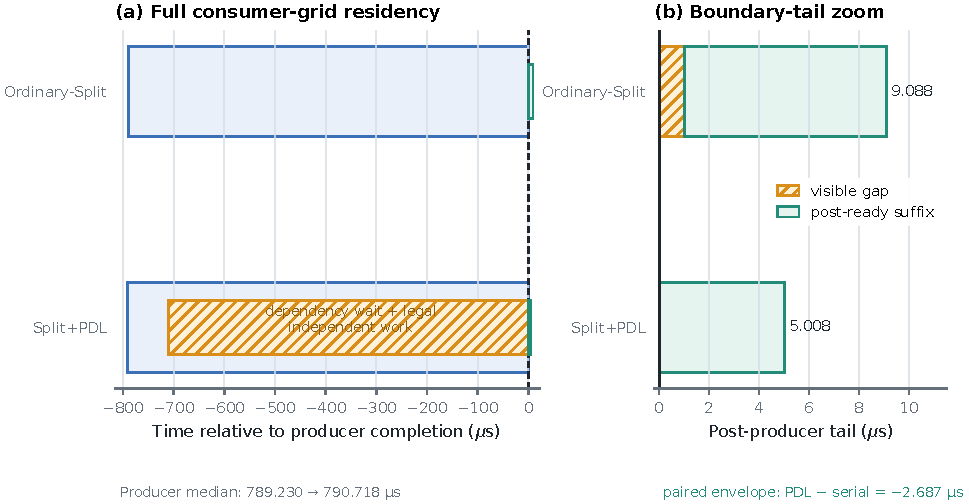
\includegraphics[width=0.98\textwidth]{Img/paper_figures/fig_pdl_nsys_timeline.pdf}
  \caption{Hazy 中心边上 Serial-Split 与 Split+PDL 的 Nsight Systems 时间结构（32K，matched binary，20 对 AB/BA）。左图将每种方案的 producer completion 对齐为零，斜线区表示 dependent grid 在 producer 完成前的驻留，其中包含 dependency wait 与合法独立工作；右图放大 producer completion 后的关键路径尾部。PDL 将 suffix tail 中位数从 $9.088\microsecond$ 降至 $5.008\microsecond$，完整 GPU envelope 的 paired-median 变化为 $-2.687\microsecond$。}
  \label{fig:pdl-nsys-timeline}
\end{figure}

代码调研与运行路径覆盖 MegaQwen、DeepGEMM MegaMoE、Mirage MPK、NVIDIA CUTLASS dependent launch 示例以及已有 PDL 实验仓库。MegaQwen 与 DeepGEMM MegaMoE 采用公开仓库的固定版本\cite{megaqwen2026,deepgemm2026}；Mirage MPK 采用论文公开版本\cite{cheng2025mpk}；PDL 接口依据 CUTLASS 示例和现有实验实现\cite{nvidia2026cutlassDependentLaunch,muuuchen2026pdlExp}。其中，\texttt{pdl\_exp} 用于接口、构建和参数路径校准；CUTLASS Example~63 与 Hazy direct-PDL binary 提供 device-side PDL 指令和真实 overlap 证据。MegaQwen 的 Qwen3-0.6B cooperative decode 已在 H800 完成可行性运行；MegaQwen MLP 真实 checkpoint trace 上已建立同 producer/consumer binary 的 serial--PDL 对照；DeepGEMM SM90 cooperative MegaMoE 已完成本机构建与官方 smoke correctness。上述代码路径为第二真实计算图和不同调度结构的交叉验证提供候选载体。

\subsection{软硬件与实验条件}

当前实验节点配备 4 张 NVIDIA H800 80GB GPUs（132 SM，compute capability 9.0），驱动版本 535.161.08；CUDA 13.2、Nsight Compute、Nsight Systems、cuobjdump、PyTorch 和完整 CUDA/C++ 构建环境已经可用。现有实验使用其中两张物理 H800 独立复验中心结果，其余设备可用于跨卡方差、并行构建和 profiler 实验。

实验资产已经包含固定上游 commits、公开 checkpoint、自然 token traces、源码与二进制 hash、SASS、逐样本 CSV/JSON、Nsys reports、NCU reports、A/A controls、正确性脚本和汇总脚本。后续工作直接在这些冻结资产上增加 admission-gated variant、layer/decode integration 和 held-out graph，能够保持先导实验与后续机制验证的可比性。
